\chapter{Preparing Atoms for Interferometry}\label{chap:atom_prep}
\section{Chapter Overview}
This chapter presents the work that went towards the initial stages of the experimental sequence, where the main objective is to prepare a sufficiently cold ensemble of \ac{rb87} in the same quantum state.


\section{Cooling in Optical Molasses}\label{sec:optical_molasses}
{\textbf{Introduce motivation here}}
A low thermal velocity means that the atoms can be interrogated for a longer time and in the case of atom interferometry, leads to a more sensitive measurement of acceleration. In addition, the thermal expansion of the ensemble leads to greater systematic phase shifts due to effects such as magnetic field gradients and laser wavefront distortions. The temperature of atoms inside the \ac{mot} is greater than desired, so further cooling is required before a strong interferometer signal can be achieved. Temperatures well below that of the Doppler limit (\sivalue{146}{\micro\kelvin} for \ac{rb87}) can be reached using the dissipative force that acts on an atom travelling through a spatially varying electric field. 

\par\noindent
This section describes the steps required to cool the atoms in a moving optical molasses, 
\begin{itemize}
    \item Introduce section
    \item mention bias fields and residual field strength
\end{itemize}

\subsection{Motivation for Launching}
The light used to drive Raman transitions during the exeperiment is launched into the chamber on two orthogonal axes of a \ac{pm} fibre. These are retro-reflected to produce two counter-propagating beams that are orthogonally polarised to the incoming ones. In the absence of \(\pi\)-polarised light, only \((\sigma^+-\sigma^+)\) or \((\sigma^--\sigma^-)\) pairs of polarised beams can drive Raman transitions. If the incoming beams are circularly polarised, then this can occur using counter-propagating pairs of beams which impart momentum \(\pm \hbar \keff\) to an atom. If an atom can be driven by either pair at each interferometer pulse, this results in two interferometer paths, as well as additional trajectories which do not interfere and hence cause a reduction in fringe visibility. Fortunately, this ``double interferometer'' problem can be avoided by making use of the velocity sensitivity of the Raman transition. Each pair has an opposite Doppler shift \(\pm \omega_D = \pm \keff.\textbf{v}\) and so their transition frequencies are separated by \(2\omega_D\). If this shift is large compared to the linewidth of the transition, then this degeneracy can be lifted so that only one pair of beams will drive Raman transitions.

\subsection{Frequency and Power Control}\label{subsec:molasses_control}
A timing diagram illustrating the power and frequency during this stage of the experiment is shown in \FigureRef{fig:molasses_timing}. After the atoms are loaded into the \ac{mot}, they are released by switching off the quadrupole field. Once this field has decayed away, the frequency and intensity of the cooling light are ramped adiabatically. The frequency of the cooling light is ramped to -25\(\Gamma\) over \sivalue{1.4}{\milli\second}. Since the repump light is generated using an \ac{eom}, the modulation frequency is simultaneously ramped up to keep this light resonant with the \trans{1}{2} transition. Additionally, the relative detuning of counter-propagating \ac{mot} beams is varied so that the atoms are cooled into a moving molasses (see~\SectionRef{subsec:moving_molasses}). After this, the intensity of the light is reduced over \sivalue{5}{\milli\second}. The response of the output \ac{aom} on the \Muquans laser was calibrated so that we could apply a voltage ramp that gives an approximately linear intensity ramp.
\begin{figure}
    \centering
    \resizebox{0.6\textwidth}{!}{\input{molasses_timing.pdf_tex}}
    \caption[Molasses stage timing diagram]{Timing diagram for the molasses stage of the experiment. After a time \(\tau_\text{a} = \sivalue{100}{\milli\second}\), the atoms are released from the \ac{mot}. The molasses sequence begins \sivalue{3}{\milli\second} later, once the magnetic field from the \ac{mot} coils has decayed away. First, the frequency of the cooling light is ramped to \(-25 \Gamma\) over \sivalue{1.4}{\milli\second}. The relative frequencies of counter-propagating \ac{mot} beams are detuned so that the atoms are cooled in a moving frame, launching them along a parabolic path (see~\SectionRef{subsec:moving_molasses}). Next, the intensity of the \ac{mot} light is reduced linearly over \sivalue{5}{\milli\second}. To measure the temperature, the atoms are left to expand for a duration of \(\tau_\text{exp}\) \sivalue{}{\milli\second}, after which they are imaged using the camera.}
    \label{fig:molasses_timing}
\end{figure}
\subsection{Launching in a Moving Molasses}\label{subsec:moving_molasses}

The configuration for launching atoms along the Raman axis is shown in \FigureRef{fig:moving_molasses}. The forward-propagating beams are blue-detuned by \(+\delta_l\) and the backward-propagating ones are red-detuned by \(-\delta_l\), so that atoms with a velocity along the beam axis of \(\vec{v} = \delta_l \lambda\) are+ resonant with both beams. The frequency of each beam is ramped from the initial value by varying the modulation frequency of its \ac{aom}. This ramp occurs slowly to ensure the atoms are adiabatically accelerated to the resonant velocity, minimising excess heating of the atoms. As there is no pair of \ac{mot} beams along the axis of the Raman beams, the \(\vec{x}\) and \(\vec{y}\) \ac{mot} beams, whose axes are nominally at 45\(^{\circ}\) to the Raman axis, are used to launch the atoms. By controlling the power and alignment of each beam, the net velocity on the atoms will be along the Raman axis. If the detuning of both pairs of beams is the same, then the velocity along the Raman axis is given by \(\vec{v_r} = \sqrt{2} \delta_l \lambda\)~\nocite{Ohshima1995}.
\begin{figure}
    \centering
    \def\svgwidth{0.6\textwidth}\input{moving_molasses.pdf_tex}
    %\resizebox{0.6\textwidth}{!}{\input{moving_molasses.pdf_tex}}
    \caption[Beam configuration for a moving molasses]{Beam configuration for a moving molasses. When counter-propagating beams are detuned from each other, the atoms are slowed to a velocity which balances the frequency of each beam. Along the vertical axis, the beams are detuned by \(\delta_v\) so that the cloud is launched upwards with a velocity \(v_z = \delta_v \lambda\). In the horizontal plane, the \(\vec{x}\) and \(\vec{y}\) beams are detuned by \(\delta_h\) so that the resultant velocity is along the Raman axis \(v_r = \sqrt{2}\delta_h\lambda\). }
    \label{fig:moving_molasses}
\end{figure}
\par\noindent
As well as launching the atoms horizontally, the atoms are launched vertically so that they do not fall as far under gravity. Since the atoms remain close to the centre of the beam, where the intensity across the cloud is more uniform, longer pulse separation times can be used before the intensity gradient causes a significant dephasing. This launch is carried out using the \ac{mot} beams that lie along the vertical \(\vec{z}\) axis. Under an appropriate choice of launch velocity, the centre-of-mass trajectory transverse to the Raman beam wavefront can be chosen to maximise the interferometer fringe visibility. This is presented in further detail in~\SectionRef{subsec:launch_contrast}. 
\par\noindent
\subsection{Imaging the Atom Cloud over Time}
Once released from the trap, the atom cloud is free to expand. Provided that there are no external forces on the atoms from electric or magnetic fields, the expansion of the cloud is determined by its thermal velocity distribution. In addition to this, the centre-of-mass moves due to its initial velocity and acceleration due to gravity. For the purposes of this discussion, it is worthwhile to consider the motion of atoms within the ensemble separately to the centre-of-mass motion as these provide a means of measuring the temperature and launch velocity, respectively. These were measured by imaging the distribution of atoms after allowing the cloud to expand in the dark for a range of expansion times. A typical atom cloud trajectory is shown in~\FigureRef{fig:launch_images}, in which the cloud was imaged up to \sivalue{76}{\milli\second} after being released from the trap.

\begin{figure}
    \centering
    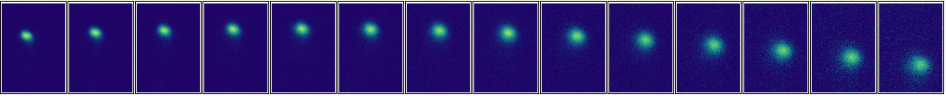
\includegraphics[width=0.8\textwidth]{molasses_launch}
    \caption[Atom cloud position after launching in a moving molasses]{A series of images showing the trajectory of the atom cloud after being cooled in a moving molasses. The first image was taken \sivalue{7}{\milli\second} after initiating the molasses and a subsequent one every \sivalue{5}{\milli\second}. Each image represents a region of interest of dimensions 1150 \(\times\) 1650 pixels that covers the spatial extent of the atom cloud during the launch.}
    \label{fig:molasses_launch}
\end{figure}
\subsubsection{Measuring the Temperature}
In thermal equilibrium, the velocity distribution of the atoms is described by a Maxwell-Boltzmann distribution
\begin{equation}
    f(v_x,v_y,v_z) = \left(\frac{m}{2\pi k_B }\right)^{3/2}e^{-\frac{m (v`_x^2+v`_y^2+v`_z^2)}{2 k_B T}}
    \label{eg:mb3D}
\end{equation}
where \(v`_i = v_i - \langle v_i \rangle\) is the difference from the average velocity. Along a single axis, the velocity distribution is obtained by integrating over the other velocity components. For the sake of notation, the following discussion uses \(x\) and \(v_x\) as labels for position and velocity, but these are interchangeable with the equivalent components along the other axes. As~\EquationRef{eg:mb3D} is a product of velocity distributions along each axis, the velocity distribution along one axis is 
\begin{equation}
    f(v_x) = \left(\frac{m}{2\pi k_B }\right)^{1/2}e^{-\frac{m (v_x-\langle v_x \rangle) ^2}{2 k_B T}}
    \label{eg:mb1D}
\end{equation}
Suppose that there are initially \(n_0 (x) \mathrm{d}x\) atoms within the region \((x, x+\mathrm{d}x)\), where \(n_0(x) = n(x, t=t_0)\) is the initial atomic density along one axis. During ballistic expansion, the atoms redestribute themselves according to their velocity. After a time \(t\) of free expansion, the position of an atom initially at \(x\) is \(x + v_x t\). 
Assuming that the number density is initially a Gaussian, with a peak number density \(n_0(x_0)\) at the centre-of-mass, the number density at later times is given by a convolution with~\EquationRef{eq:mb1D}
\begin{equation}
        n(x,t) = \int n_0(x_0) \left(\frac{m}{2\pi k_B}\right)^{1/2} e^{-\frac{m (v_x-\langle v_x \rangle)^2}{2 k_B T}} e^{-\frac{(x+v_x t - x_0)^2}{2\sigma_0^2}} \mathrm{d}v_x
        \label{eq:density_time}
\end{equation}
where \(\sigma_0\) is the \(1/e^2\) initial width of the cloud. As a convolution of two Gaussians, \EquationRef{eq:density_time} is also a Gaussian, with a \(1/e^2\) width given by
\begin{equation}
    \sigma(t)^2 = \sigma_0^2 + \frac{k_B T}{m} t^2
    \label{eq:expansion_width}
\end{equation}
\par\noindent
\FigureRef{fig:molasses_temperature} shows the measured cloud width over a range of expansion times. The inset shows a typical density profile along each axis, obtained by imaging the cloud on a camera, as previously described in~\SectionRef{eq:imaging}. For the purposes of measuring the temperature, the total atom number and the initial cloud size are not important, so no attempt was made to estimate these. The initial measurement was made \sivalue{7}{\milli\second} after the end of the molasses to allow for enough time to re-lock the laser to \(-0.5\Gamma\) below the \trans{2}{3} transition and align the bias field to the \(\vec{z}\) axis so that the atoms could be optically pumped into the \(\ket{2,2}\) state. At each measurement time, a non-linear least squares fit to~\EquationRef{eq:density_time} along each axis was carried out to estimate the width of the cloud. Then, a least squares linear fit was used to estimate the temperature along each axis from the gradient, as per~\EquationRef{eq:expansion_width}. The measured temperature along the horizontal and vertical axes of the camera was \(T_x = \sivalue{6.37 \pm0.15}{\micro\kelvin}\) and \(T_y = \sivalue{6.38\pm0.12}{\micro\kelvin}\), respectively.  

\begin{figure}
    \centering
    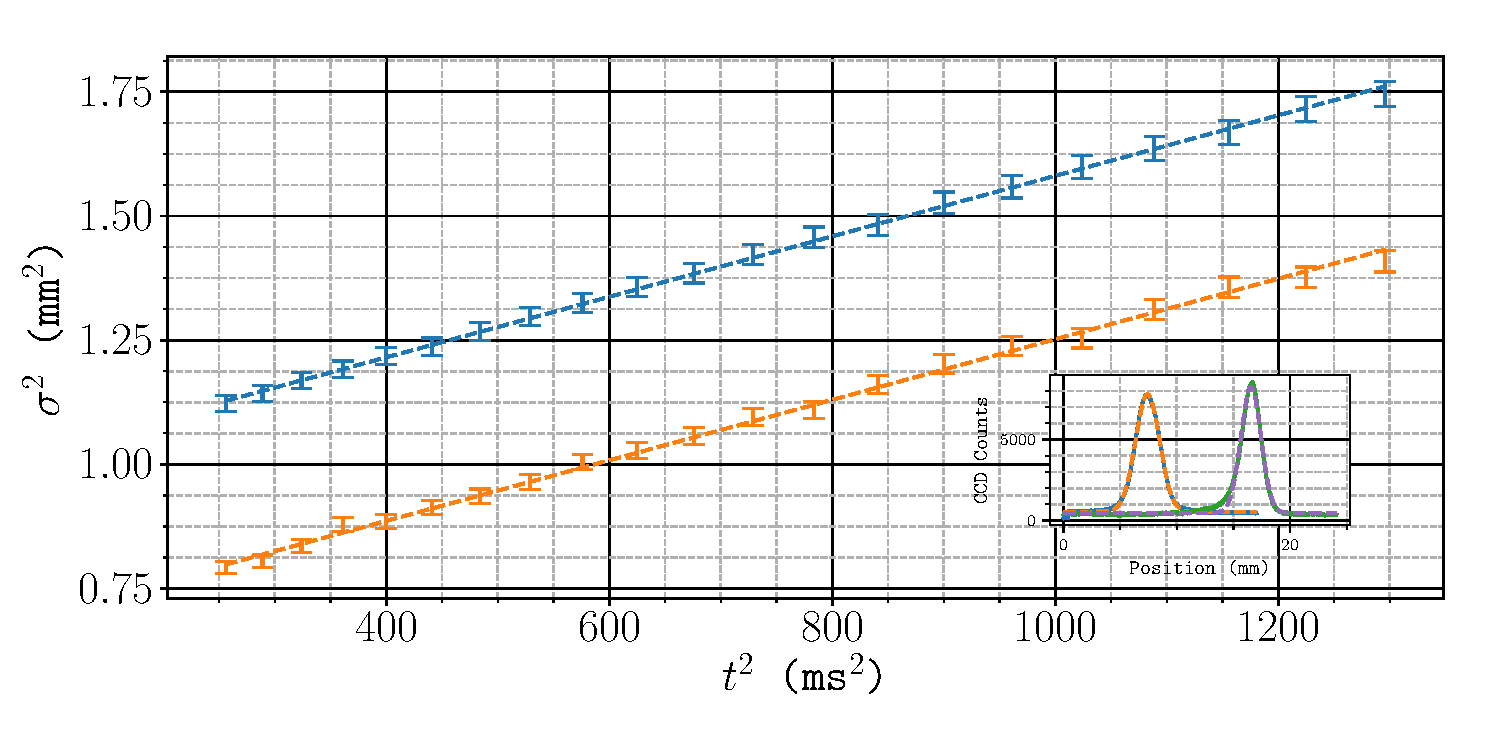
\includegraphics[width=0.8\textwidth]{temperature_launch}
    \caption[Temperature measurement using ballistic expansion]{Atom cloud temperature using a ballistic expansion measurement. After molasses, the cloud is left to expand in the dark and in a region of close to zero magnetic field. A least-squares linear fit of \(\sigma(t)^2\) is used to estimate the temperature using~\EquationRef{eg:expansion_width}. The inset shows a typical density profile from a single image, obtained by integrating the signal from a CCD camera along the two axes of the the sensor. The gradient from the fits for the horizontal (blue) and vertical (orange) axes are  \(T_x = \sivalue{6.38 \pm0.15}{\micro\kelvin}\) and \(T_y = \sivalue{6.38\pm0.12}{\micro\kelvin}\).}
    \label{fig:molasses_temperature}
\end{figure}

\subsubsection{Measuring the Launch Trajectory}
The same method used to measure the temperature of the cloud can also be used to measure the position of the centre-of-mass. In this case, the quantity of interest is \(\langle x(t)\rangle\). Since the cloud is in free-fall, the trajectory for the centre-of-mass is then given by the well-known equation-of-motion for a particle moving under constant acceleration
\begin{equation}
    \langle x(t) \rangle = \langle x(0) \rangle + v_x t + \frac{1}{2} a_x t^2
    \label{eq:position_free}
\end{equation}
where \(v_i\) is the initial velocity along the given axis and \(a_i\) is the acceleration.
\par\noindent
To launch the atoms both vertically and horizontally (along the axis parallel with the Raman light), the \((z_+, z_-)\) \acp{aoms} were ramped so that the relative frequency difference between each beam was \(2\times\)\sivalue{320}{\kilo\hertz} and the \(x\) and \(y\) \ac{aom} frequencies were ramped to give a frequency difference of \(2\times \sivalue{75}{\kilo\hertz}\) between the horizontal \ac{mot} beams. \FigureRef{fig:molasses_launch} is a plot of the measured centre-of-mass position along the horizontal and vertical camera axes over time. A linear least-squares fit to~\EquationRef{eq:position_free} gives a vertical launch quantities of \(v_v = \sivalue{25.0\pm0.35}{\centi\meter\per\second}\) and \(a_v = \sivalue{-9.40\pm0.075}{\metre\per\second\squared}\) and \(v_h = \sivalue{7.39\pm0.21}{\centi\meter\per\second}\) and \(a_h = \sivalue{-0.31\pm0.052}{\metre\per\second\squared}\) along the horizontal axis. 
\begin{figure}
    \centering
    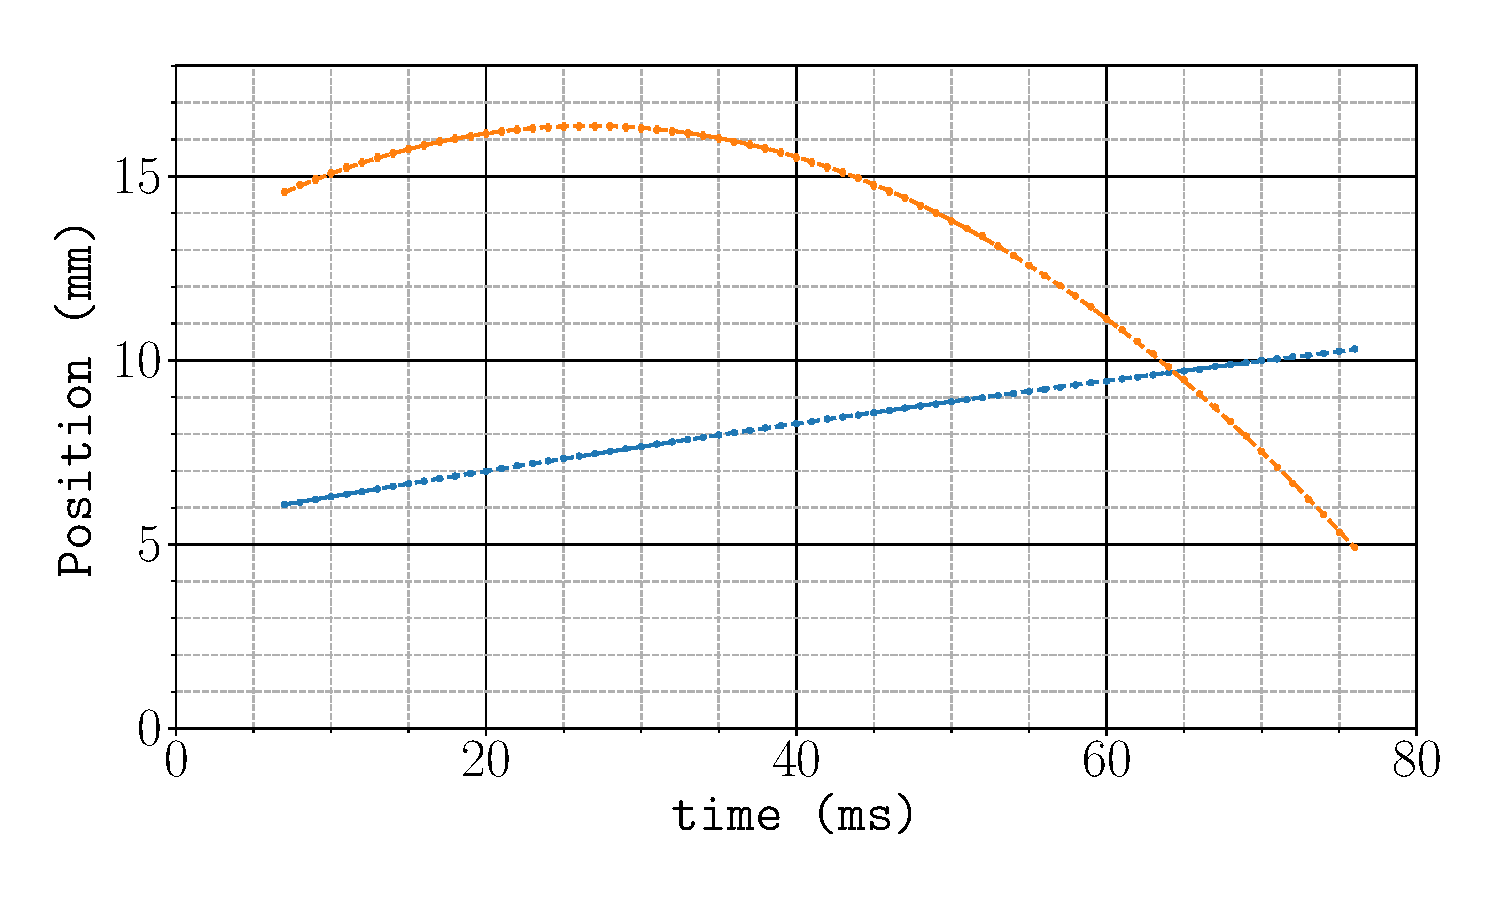
\includegraphics[width=0.8\textwidth]{molasses_position}
    \caption[Atom cloud centre-of-mass over time]{Measured centre-of-mass position over time. The horiztonal component of the position is shown in blue and the vertical in orange. Each trajectory is fit to~\EquationRef{eq:position_free} to estimate the launch velocity. The best-fit values are \(v_v = \sivalue{25.0\pm0.35}{\centi\meter\per\second}\) and \(a_v = \sivalue{-9.40\pm0.075}{\metre\per\second\squared}\) along the vertical axis and \(v_h = \sivalue{7.39\pm0.21}{\centi\meter\per\second}\) and \(a_h = \sivalue{-0.31\pm0.052}{\metre\per\second\squared}\) along the horizontal.}
    \label{fig:molasses_position}
\end{figure}
\par\noindent
When compared to the expected velocities from the detunings, \(v^{(l)}_v = \sivalue{24.96}{\centi\metre\per\second}\) and  \(v^{(l)}_h = \sivalue{5.85}{\centi\metre\per\second}\), the measured horizontal velocity is far greater than expected. This can be explained by a residual magnetic field, that is not cancelled using the bias coils. In the presence of a magnetic field, atoms cooled in an optical molasses are decelerated to a velocity at which the Zeeman shift is cancelled by the Doppler shift. This \ac{vsr} depends on the orientation of the magnetic field to the polarisation of the light. Previous work studying this effect on a one-dimensional optical molasses has identified a \ac{vsr} of \(v_\text{res}^{(1)} = - \mu_B g_F B/\hbar k\) when the magnetic field is aligned with the wave-vector of the light \cite{VanderStraten1993}. When the field is aligned at an arbitrary angle a second resonance at \(v_\text{res}^{(2)} = - \mu_B g_F B/2\hbar k\) is present, due to additional \(\left(\sigma^{\pm}-\pi\right)\) transitions~\cite{Chang2002}. `As discussed later in~\SectionRef{subsec:raman_mems}, the \ac{mems} accelerometer mounted behind the retro-reflecting mirror contains a permanent magnet.  

\section{State Preparation}\label{sec:state_prep}
\subsection{Schemes for Preparation}
\subsection{Optical Pumping Scheme} 
\subsection{Including Microwave Transitions}
\subsubsection{Wind-Freak Synthesiser}\label{subsec:windfreak}

\subsection{Blow-Away}\label{subsec:blow_away}